The name of the fist prototype, which was developed in Valencia, is Tritium-IFIC 0 and it was the proof where we could check that we were able to detect tritium in water samples with this technology. This protoype is shown in the figure \ref{fig:Tritium_IFIC_0}.

\begin{figure}[htb]
\centering
{
%\subfloat[Front view]{
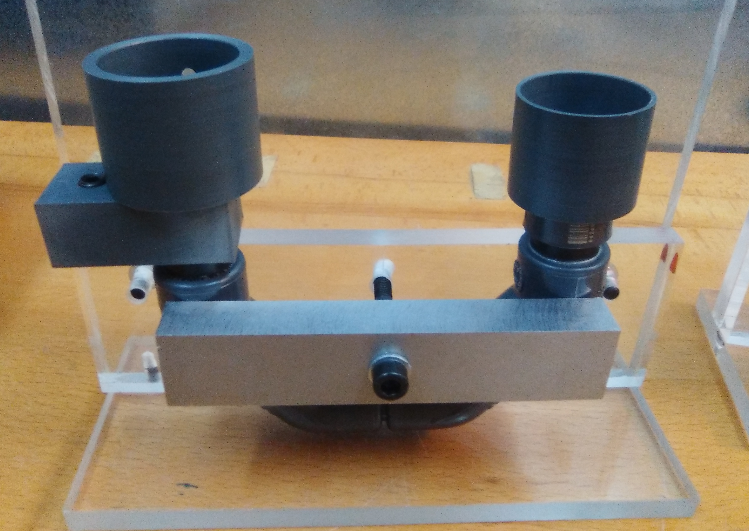
\includegraphics[scale=0.25]{Prototipodelantetapon.png} 
}
{
%\subfloat[Back view]{
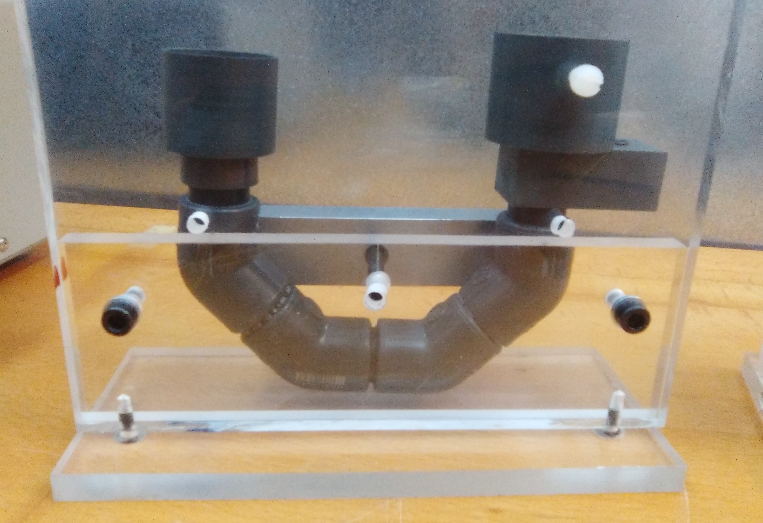
\includegraphics[scale=0.25]{PrototipoDetrastapon.png} 
}
\caption{Tritium-IFIC 0 prototype. Front view (left) and back view (right) \label{fig:Tritium_IFIC_0}}
\end{figure} 

This prototype contains $35$ scintillating fibers read out by two PMTs in coincidence, which was bought from Hamamatsu company, model R8520. 

These fibers were contained in a PVC vessel because it is a safe material widely used in plumbing. On top of that, as you can see in the figure \ref{fig:Tritium_IFIC_0}, it has a U-shape because it is safer. 

Two identical prototypes were built with internal diameter of $15~\mm $ and an internal volume of $39~\cm^2$, which was verified with various fill tests. The first prototype, which was used for getting the tritium signal of the system, was filled with tritium solution with high activity ($53.385~\mega\becquerel/\liter$) and the other prototype, which was used for getting the background signal of the system, was filled with hiper-pure water. 

These prototypes is hold with a methalic and steel structure, which was constructed in the IFIC workshop. The electronic circuit used for processing the signals of each circuit was the same and its electronic scheme is shown in the figure \ref{fig:Electronic_scheme}.

\begin{figure}[htb]
\centering
{
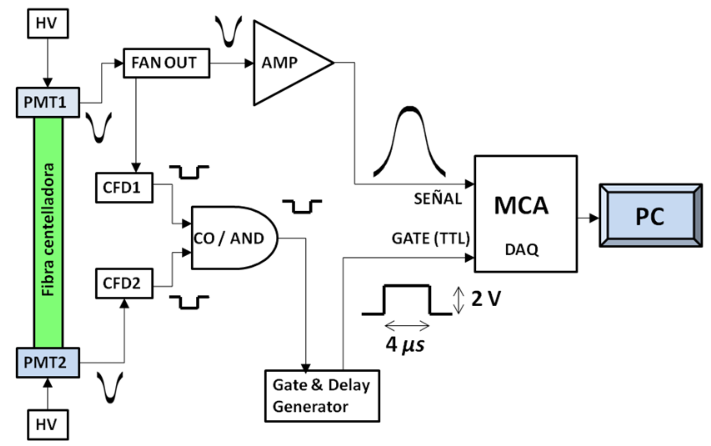
\includegraphics[scale=0.4]{Esquemaelectronico.png} 
}
\caption{Electronic scheme used for analysing the signal of Tritium-IFIC 0 prototype \label{fig:Electronic_scheme}}
\end{figure} 

It is based on several NIM technology modules with which we amplify the signal of the detector and make coincidence between both PMTs in order to remove the electronic noise of the PMTs. 

The measurement obtained from both prototypes are shown in the figure \ref{fig:SignalsTritiumIFIC0} and the difference between both signals, which correspond to the tritium signal, are shown in the \ref{fig:ClearSignalTritiumIFIC0}. 

\begin{figure}[htbp]
\centering
\subfigure[Signal and Background of Tritium-IFIC 0 \label{fig:SignalsTritiumIFIC0}]{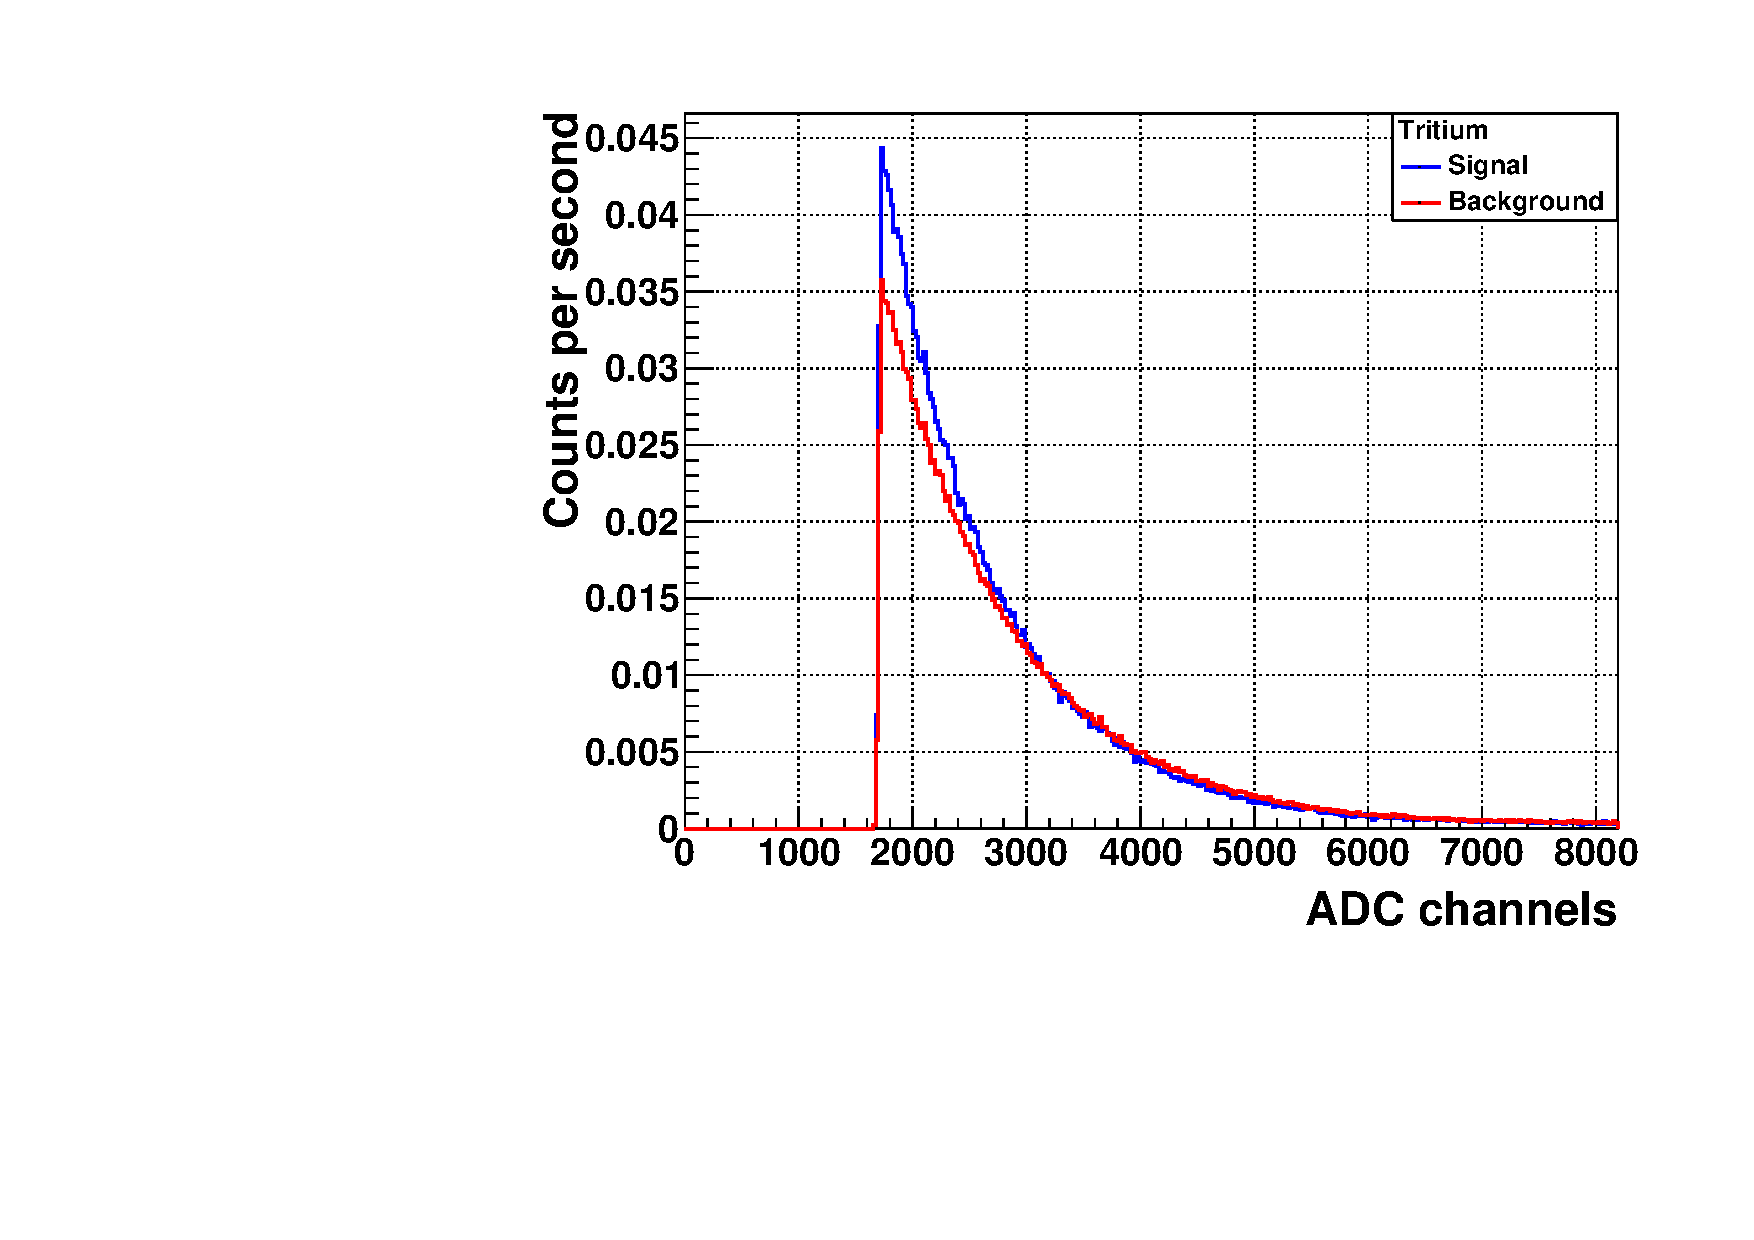
\includegraphics[width=77mm]{./Figuras/tritio-fondo_Tritium0.pdf}}
\subfigure[Clear signal of tritium \label{fig:ClearSignalTritiumIFIC0}]{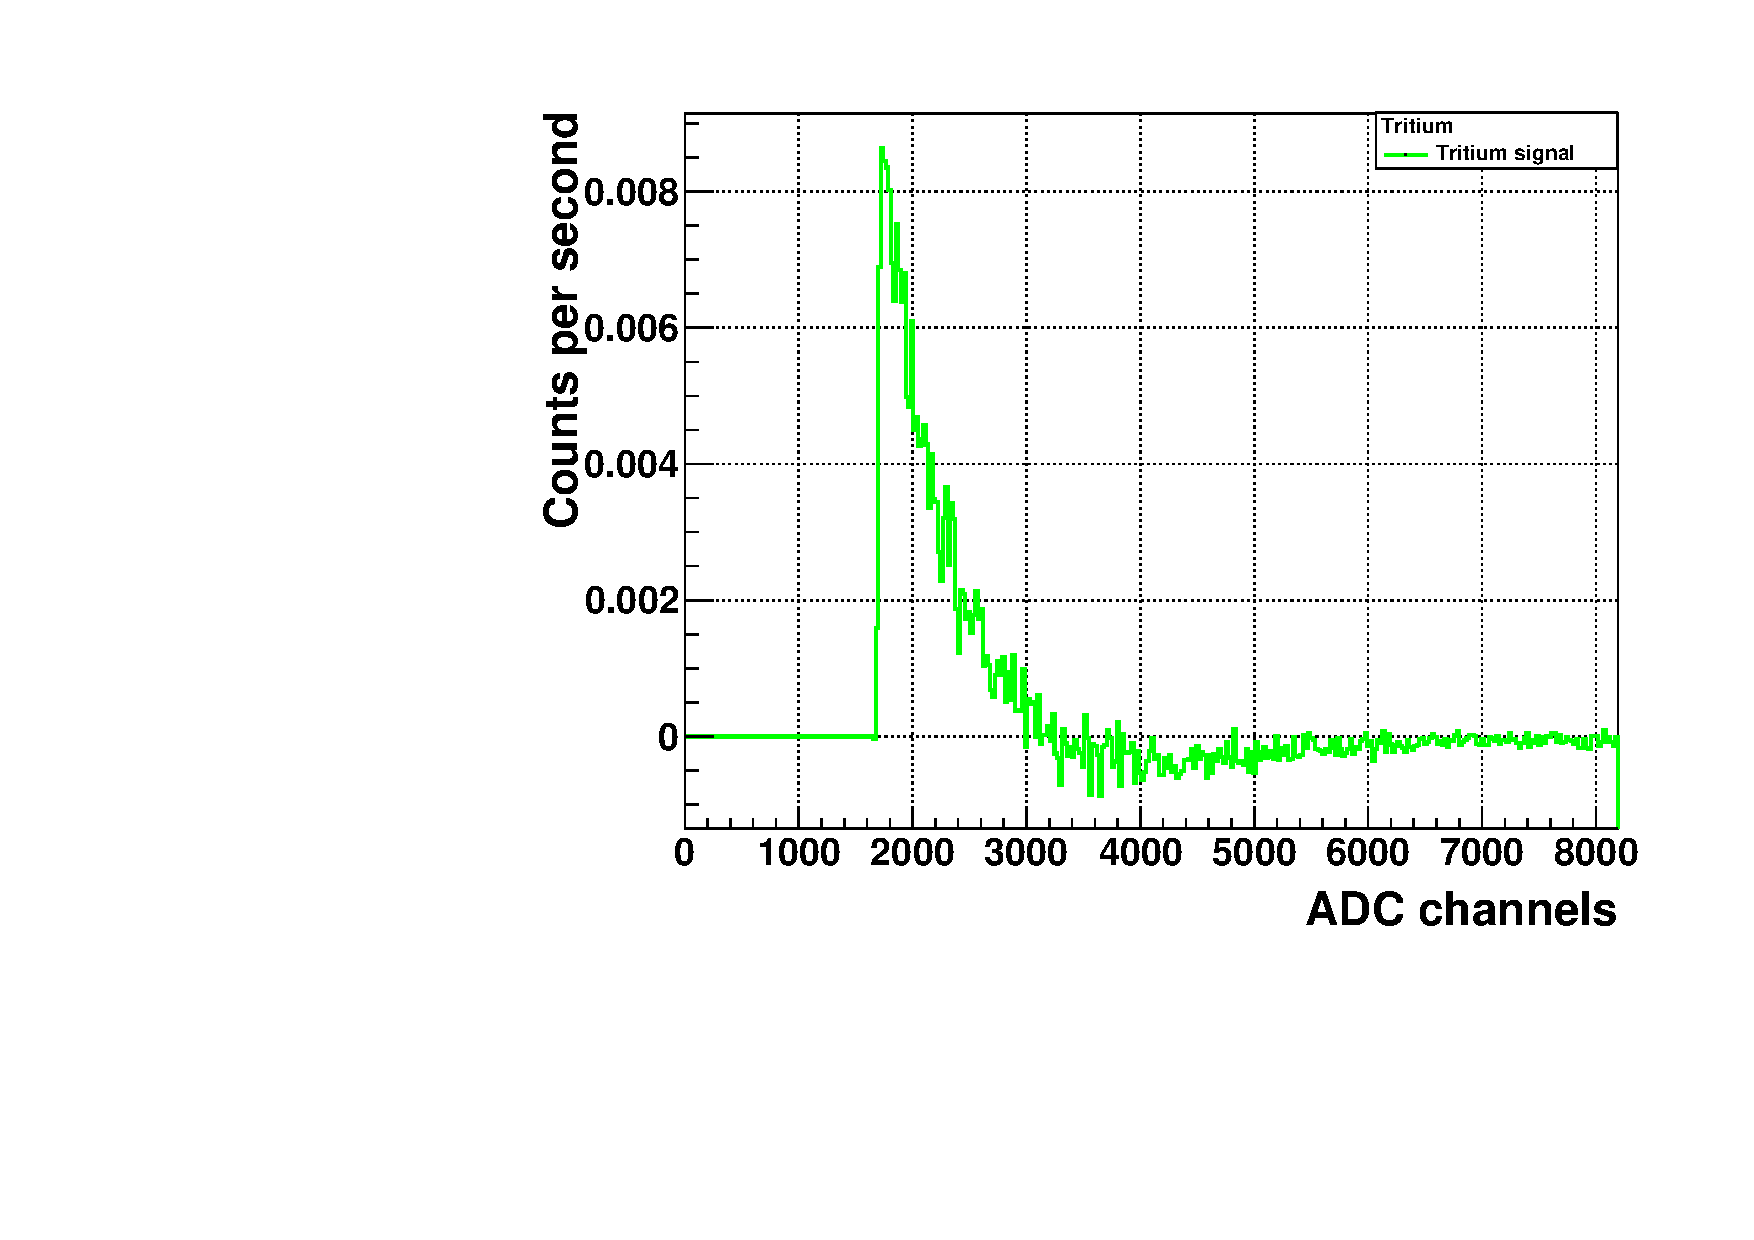
\includegraphics[width=77mm]{./Figuras/tritiumsignal_Tritium0.pdf}}
\caption{Signals of Tritium-IFIC 0 prototype.} \label{fig:Tritium_IFIC_0_Signals}
\end{figure}

In this experience we have obtained $0.199$ counts per second for this activity, which means that the effiecincy of our detector is $ \varepsilon_{det} = 3.728 \cdot 10^{-6}~(\ce{counts}/\sec)/(\kilo\becquerel/\liter)$. We know that the efficiency of this type of detectors scales with the active surface so we can obtain the specific efficiency. It is the efficiency normalized to the active surface of our detector ($A_{suf} = 219.8~\cm^2$) whose value is $ \varepsilon_{esp} = \varepsilon_{det}/A_{suf} =  1.695 \cdot 10^{-8}~(\ce{counts}/\sec)/(\cm^2\kilo\becquerel/\liter)$. 

This value of specific efficiency is two orders smaller than the one get with other similar detectors (reference of the thesis) so we looked for the reason of this fact. 

We viewed the surface of the scintillator fibers under the electron microscope and, as you can see in the figure \ref{fig:FiberSurfaceElectronMicroscope}, we found that this surface was not as good as we though. 

\begin{figure}[htbp]
\centering
%\subfigure[]
{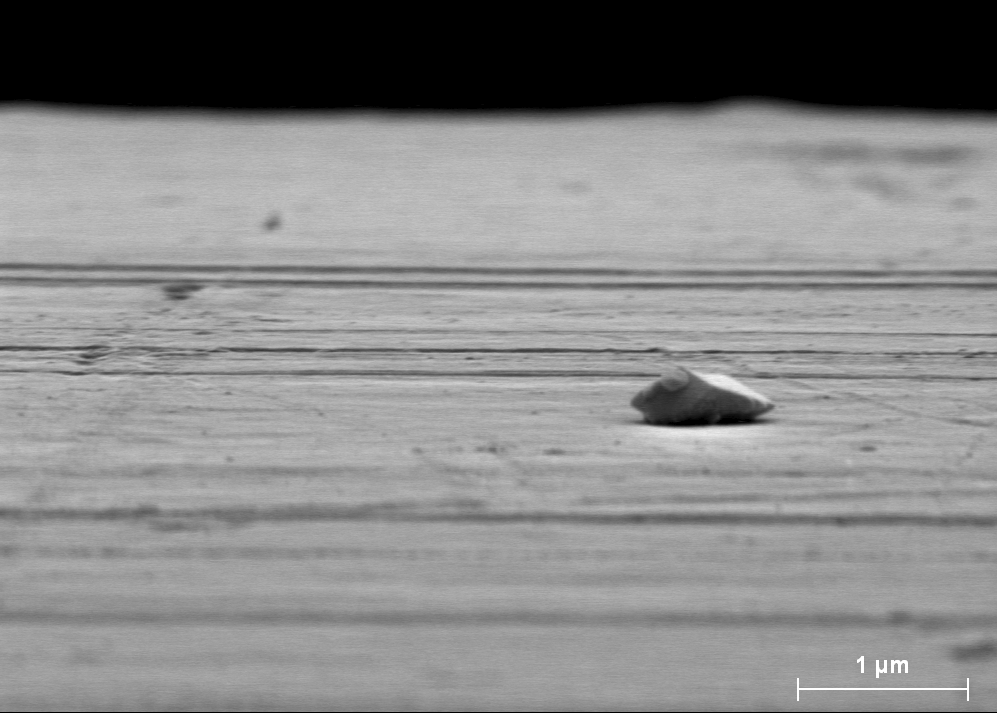
\includegraphics[width=70mm]{./Figuras/sinclad_3_SE.png}}\hspace{10mm}
%\subfigure[]
{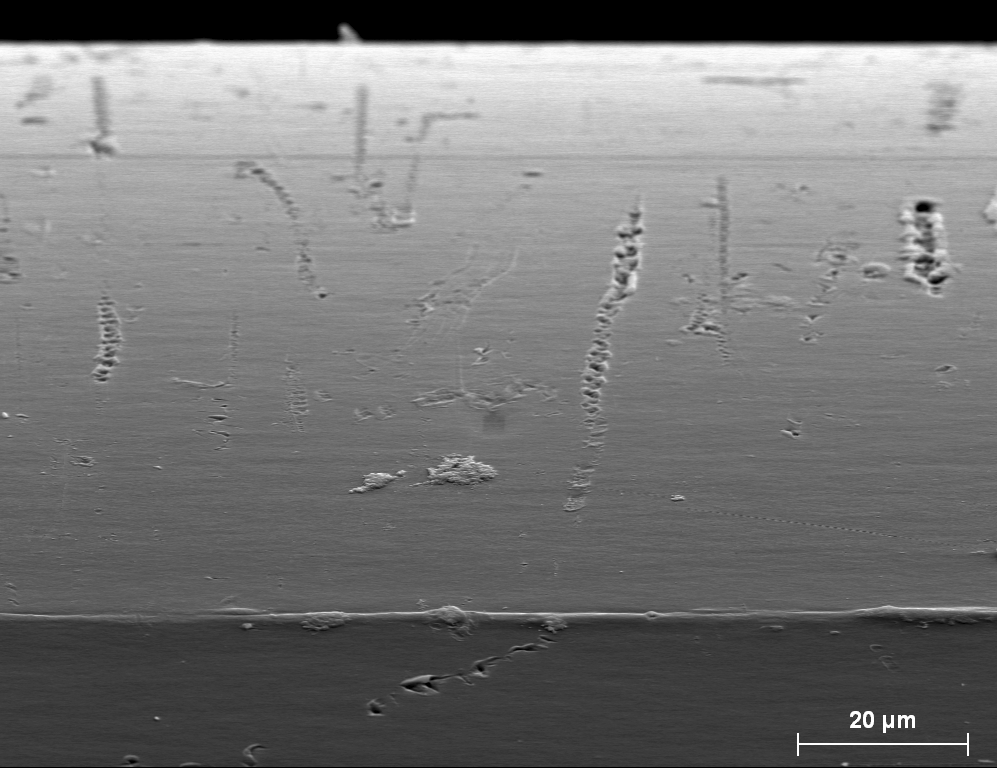
\includegraphics[width=70mm]{./Figuras/sinclad_6_SE.png}}
\caption{Suface of scintillating fibers under electron microscope.} \label{fig:FiberSurfaceElectronMicroscope}
\end{figure}

It has a lot of irregularities and, due to that, we had a loss of light, overall, in the curve of the fibers. It was checked with a simply set-up which is shown in the figure \ref{fig:CurveLight}.

\begin{figure}[htb]
\centering
{
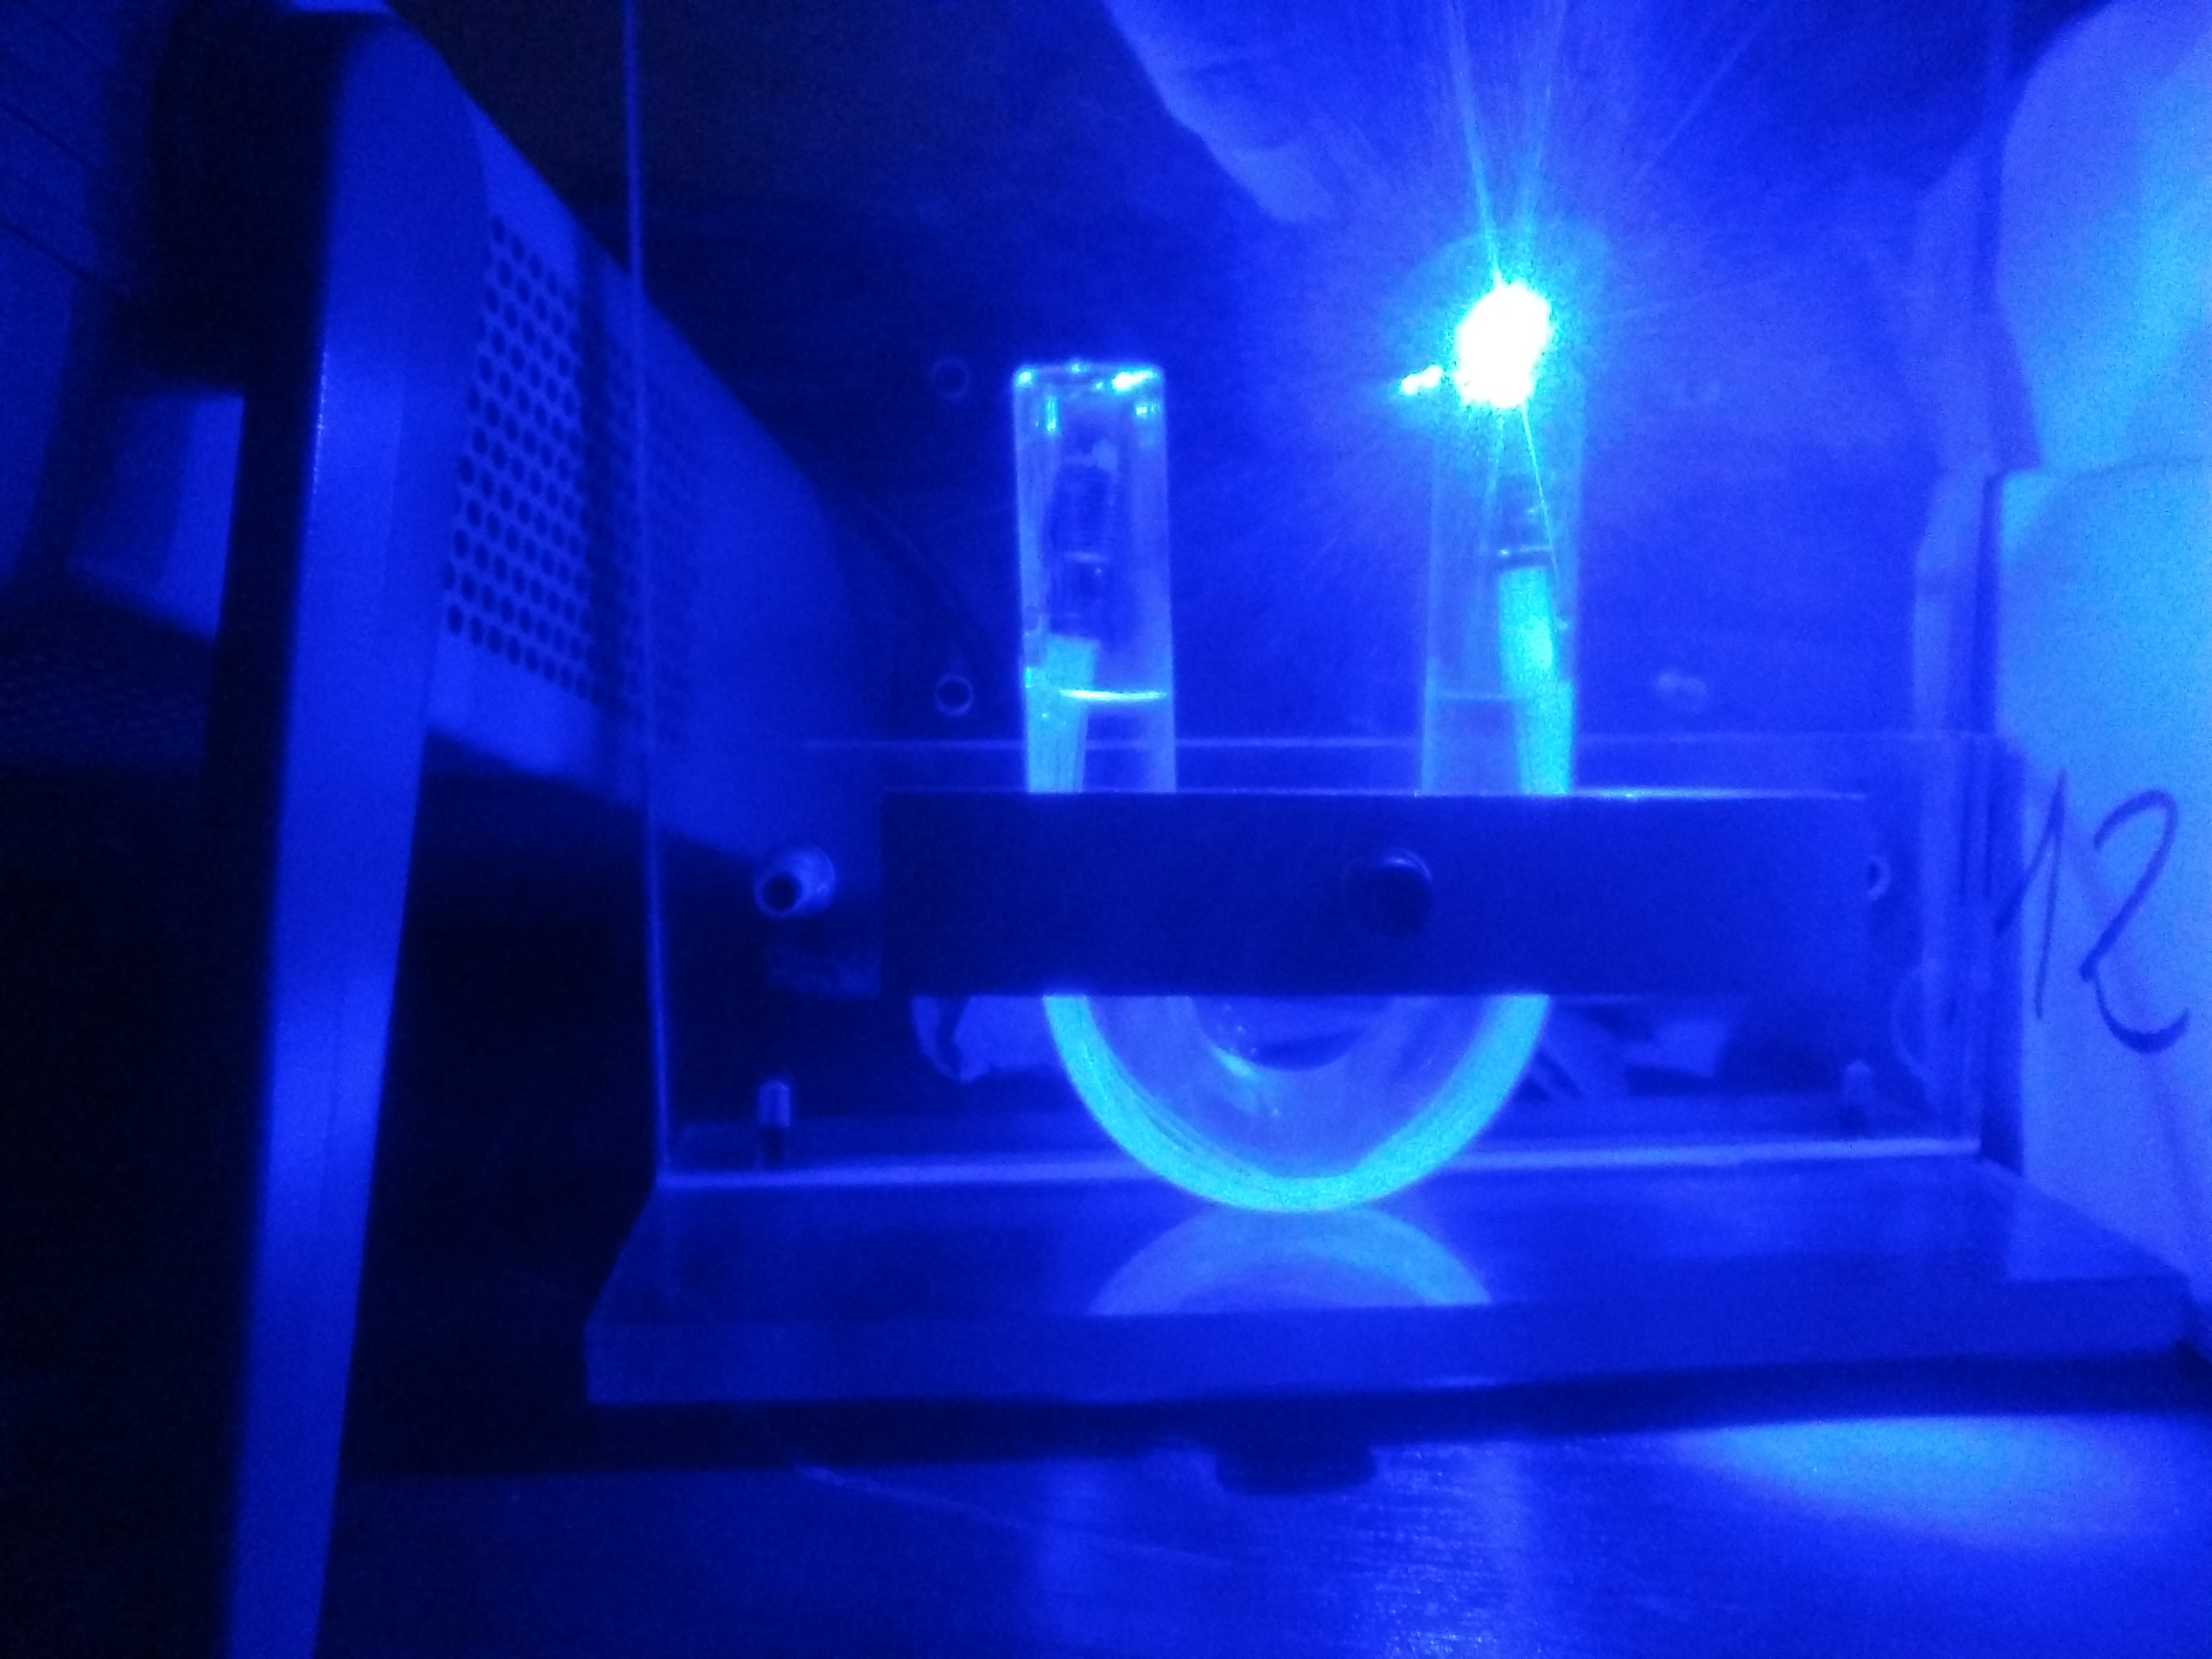
\includegraphics[scale=0.12]{CurveLight.jpg} 
}
\caption{Loss of light due to the curve of the fibers. \label{fig:CurveLight}}
\end{figure}

As a result of this photons losing, we loss some events and, by extension, the efficiency of our detector will be smaller.

Another possible reason for this low efficiency is due to the strong bonding of the fibers. As you can see in the figure \ref{fig:Metalic_piece_bunch}, there are two metalic pieces in each fiber bunch, which join the fibers strongly and, due to that, the water cannot cross among these fibers. It produces that the active area of our detector is smaller and, thus, the specific efficiency of our detector are higher.

\begin{figure}[htbp]
\centering
{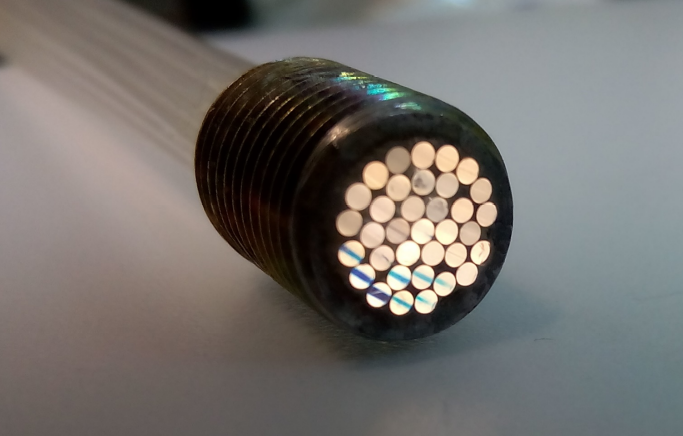
\includegraphics[width=70mm]{./Figuras/Metalic_piece_bunch_fibers.png}}\hspace{10mm}
{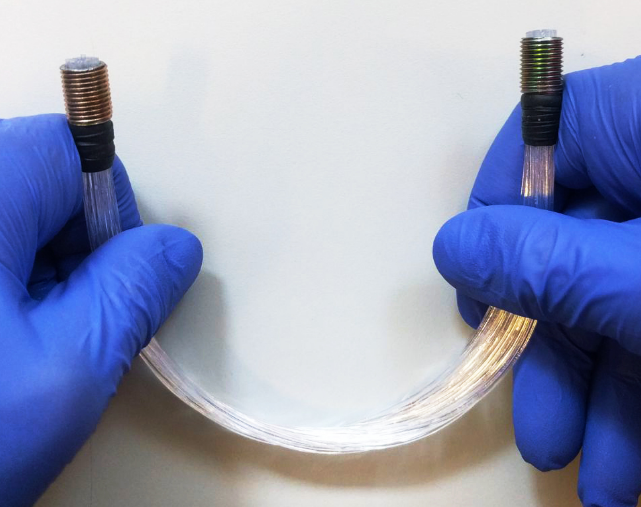
\includegraphics[width=70mm]{./Figuras/bunch_fibers.png}}
\caption{Metal pieces used in the fiber bunch of Tritium-IFIC 0 prototype} \label{fig:Metalic_piece_bunch}
\end{figure}
